\documentclass{article}

\usepackage[margin=1in]{geometry}
\usepackage{amsmath,amsthm,amssymb}
\usepackage{array,multirow}
\usepackage{bbm, enumerate, tikz}

\let\originalleft\left
\let\originalright\right
\renewcommand{\left}{\mathopen{}\mathclose\bgroup\originalleft}
\renewcommand{\right}{\aftergroup\egroup\originalright}

\newcommand{\n}[1]{\multicolumn{1}{|c|}{#1}}
\newcommand{\set}[1]{\left\{#1\right\}}

\newtheorem{theo}{Theorem}[subsection]
\newtheorem{definition}[theo]{Definition}
\newtheorem{conjecture}[theo]{Conjecture}
\newtheorem{example}[theo]{Example}
\newtheorem{exercise}[theo]{Exercise}
\newtheorem{note}[theo]{Note}

\begin{document}

\title{Permutation statistics}
\author{Peter Kagey}

\maketitle
\section{Symmetric Polynomials}
% \begin{definition}
  % A symmetric polynomial ...
% \end{definition}
\subsection{Monomial}
\begin{definition}[Monomial symmetric polynomial]
  % Let $\lambda = (\lambda_1, \cdots, \lambda_\ell)$ be a partition of $n$, then all degree $n$ symmetric polynomials
  % can be written with basis
  Let $\lambda = (\lambda_1, \cdots, \lambda_\ell)$ with be a partition, then
  the monomial symmetric polynomial $m_\lambda$ on $m \geq \ell$ variables is
  defined to be
  \[
    m_\lambda(x_1, x_2, \cdots, x_m)
    = \sum_{\sigma \in S_\infty}x_{\sigma(1)}^{\lambda_1} \cdots x_{\sigma(\ell)}^{\lambda_\ell}.
  \]
\end{definition}
\begin{definition}[Monomial basis]
  Let $\lambda = (\lambda_1, \cdots, \lambda_\ell)$ be a partition of $n$, then all degree $n$ symmetric polynomials
  can be written with basis \[
    \set{m_\lambda(x_1, x_2, \cdots)
    = \sum_{\sigma \in S_m}x_{\sigma(1)}^{\lambda_1} \cdots x_{\sigma(\ell)}^{\lambda_\ell}
    : |\lambda| = n \text{ and } \ell \leq m}.
  \]
\end{definition}
\begin{example}
  The symmetric polynomial \[
    f(x_1, x_2, x_3) = -x_1^2 + 4x_1x_2 + 4x_1x_3 - x_2^2 + 4x_2x_3 - x_3^2
  \] can be written in the monomial basis as \[
    f(x_1, x_2, x_3) = 4m_{(1,2)} - m_{(2)}.
  \]
\end{example}
\begin{exercise}
  Show that \[
    \mathfrak{B}_m = \set{m_\lambda(x) : \lambda \text{ a partition of } n \text{ with at most } m \text{ rows} }
  \] is indeed a basis for The space of homogenous symmetric polynomials of
  degree $n$ in $m$ variables.
  \begin{proof}
    Of course, $m_\lambda(x)$ is itself a symmetric polynomial, and the
    difference of symmetric polynomials is itself symmetric. Thus the proof
    will proceed inductively: let $f(x)$ be an arbitrary symmetric polynomial,
    and look at the leading term \[
      f(x) = \alpha x_{i_1}^{\lambda_1}\cdots x_{i_\ell}^{\lambda_\ell} + \cdots.
    \] subtract $\alpha m_\lambda(x)$, and you get a polynomial with strictly
    fewer terms, by symmetry. Since a symmetric polynomial only has a finite
    number of terms, after a finite number of steps, this constructs $f$ as sums of polynomials in $\mathfrak{B}_m$.
    \\
    It is clear that $\mathfrak{B}_m$ spans the space of such symmetric
    polynomials, so the only thing left to check that $\mathfrak{B}_m$ is
    linearly independent. However, since every $m_\lambda(x)$ is nonzero when
    $\lambda$ has fewer then $m$ rows, and any linear combination of nonzero
    monomial symmetric polynomials is distinct ``on inspection'',
    $\mathfrak{B}_m$ is linearly independent.
  \end{proof}
\end{exercise}
\subsection{Schur}
\begin{definition}[Schur polynomial]
  Fulton defines the Schur polynomial to be \[
    s_\lambda(x) = \sum_{T \text{ shape }\lambda} x^T,
  \] where the sum is over all Semi-standard Young Tableaux.
\end{definition}
\begin{example}
  \begin{align*}
  s_{(3,1)}(x_1, x_2, x_3) &=
  \underbrace{x_1^3x_2}_{
  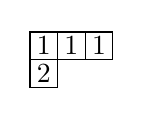
\begin{tikzpicture}[scale=0.35, baseline=-0.5ex]
    \draw (0,0) rectangle (3,1);
    \draw (0,-1) rectangle (1,0);
    \draw (1,-1)--(1,1);
    \draw (2,0)--(2,1);
    \node at (0.5,0.5) {$1$};  \node at (1.5,0.5) {$1$}; \node at (2.5,0.5) {$1$};
    \node at (0.5,-0.5) {$2$};
  \end{tikzpicture}
  }
  +
  \underbrace{x_1^3x_3}_{
  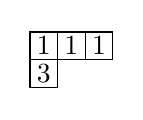
\begin{tikzpicture}[scale=0.35, baseline=-0.5ex]
    \draw (0,0) rectangle (3,1);
    \draw (0,-1) rectangle (1,0);
    \draw (1,-1)--(1,1);
    \draw (2,0)--(2,1);
    \node at (0.5,0.5) {$1$};  \node at (1.5,0.5) {$1$}; \node at (2.5,0.5) {$1$};
    \node at (0.5,-0.5) {$3$};
  \end{tikzpicture}
  }
  +
  \underbrace{x_1^2x_2^2}_{
  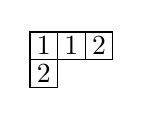
\begin{tikzpicture}[scale=0.35, baseline=-0.5ex]
    \draw (0,0) rectangle (3,1);
    \draw (0,-1) rectangle (1,0);
    \draw (1,-1)--(1,1);
    \draw (2,0)--(2,1);
    \node at (0.5,0.5) {$1$};  \node at (1.5,0.5) {$1$}; \node at (2.5,0.5) {$2$};
    \node at (0.5,-0.5) {$2$};
  \end{tikzpicture}
  }+
  \underbrace{x_1^2x_2x_3}_{
  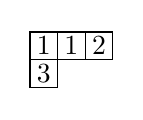
\begin{tikzpicture}[scale=0.35, baseline=-0.5ex]
    \draw (0,0) rectangle (3,1);
    \draw (0,-1) rectangle (1,0);
    \draw (1,-1)--(1,1);
    \draw (2,0)--(2,1);
    \node at (0.5,0.5) {$1$};  \node at (1.5,0.5) {$1$}; \node at (2.5,0.5) {$2$};
    \node at (0.5,-0.5) {$3$};
  \end{tikzpicture}
  }
  +
  \underbrace{x_1^2x_2x_3}_{
  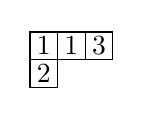
\begin{tikzpicture}[scale=0.35, baseline=-0.5ex]
    \draw (0,0) rectangle (3,1);
    \draw (0,-1) rectangle (1,0);
    \draw (1,-1)--(1,1);
    \draw (2,0)--(2,1);
    \node at (0.5,0.5) {$1$};  \node at (1.5,0.5) {$1$}; \node at (2.5,0.5) {$3$};
    \node at (0.5,-0.5) {$2$};
  \end{tikzpicture}
  }
  +
  \underbrace{x_1^2x_3^3}_{
  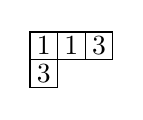
\begin{tikzpicture}[scale=0.35, baseline=-0.5ex]
    \draw (0,0) rectangle (3,1);
    \draw (0,-1) rectangle (1,0);
    \draw (1,-1)--(1,1);
    \draw (2,0)--(2,1);
    \node at (0.5,0.5) {$1$};  \node at (1.5,0.5) {$1$}; \node at (2.5,0.5) {$3$};
    \node at (0.5,-0.5) {$3$};
  \end{tikzpicture}
  }
  +
  \underbrace{x_1x_2^3}_{
  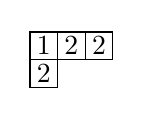
\begin{tikzpicture}[scale=0.35, baseline=-0.5ex]
    \draw (0,0) rectangle (3,1);
    \draw (0,-1) rectangle (1,0);
    \draw (1,-1)--(1,1);
    \draw (2,0)--(2,1);
    \node at (0.5,0.5) {$1$};  \node at (1.5,0.5) {$2$}; \node at (2.5,0.5) {$2$};
    \node at (0.5,-0.5) {$2$};
  \end{tikzpicture}
  }
  +
  \underbrace{x_1x_2^2x_3}_{
  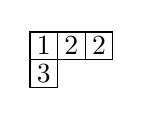
\begin{tikzpicture}[scale=0.35, baseline=-0.5ex]
    \draw (0,0) rectangle (3,1);
    \draw (0,-1) rectangle (1,0);
    \draw (1,-1)--(1,1);
    \draw (2,0)--(2,1);
    \node at (0.5,0.5) {$1$};  \node at (1.5,0.5) {$2$}; \node at (2.5,0.5) {$2$};
    \node at (0.5,-0.5) {$3$};
  \end{tikzpicture}
  } \\
  &\hspace{1cm}+
  \underbrace{x_1x_2^2x_3}_{
  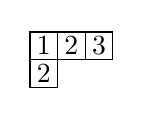
\begin{tikzpicture}[scale=0.35, baseline=-0.5ex]
    \draw (0,0) rectangle (3,1);
    \draw (0,-1) rectangle (1,0);
    \draw (1,-1)--(1,1);
    \draw (2,0)--(2,1);
    \node at (0.5,0.5) {$1$};  \node at (1.5,0.5) {$2$}; \node at (2.5,0.5) {$3$};
    \node at (0.5,-0.5) {$2$};
  \end{tikzpicture}
  }
  +
  \underbrace{x_1x_2x_3^2}_{
  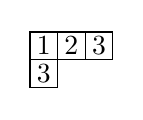
\begin{tikzpicture}[scale=0.35, baseline=-0.5ex]
    \draw (0,0) rectangle (3,1);
    \draw (0,-1) rectangle (1,0);
    \draw (1,-1)--(1,1);
    \draw (2,0)--(2,1);
    \node at (0.5,0.5) {$1$};  \node at (1.5,0.5) {$2$}; \node at (2.5,0.5) {$3$};
    \node at (0.5,-0.5) {$3$};
  \end{tikzpicture}
  }
  +
  \underbrace{x_1x_2x_3^2}_{
  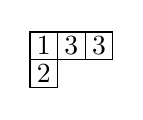
\begin{tikzpicture}[scale=0.35, baseline=-0.5ex]
    \draw (0,0) rectangle (3,1);
    \draw (0,-1) rectangle (1,0);
    \draw (1,-1)--(1,1);
    \draw (2,0)--(2,1);
    \node at (0.5,0.5) {$1$};  \node at (1.5,0.5) {$3$}; \node at (2.5,0.5) {$3$};
    \node at (0.5,-0.5) {$2$};
  \end{tikzpicture}
  }
  +
  \underbrace{x_1x_3^3}_{
  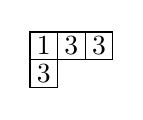
\begin{tikzpicture}[scale=0.35, baseline=-0.5ex]
    \draw (0,0) rectangle (3,1);
    \draw (0,-1) rectangle (1,0);
    \draw (1,-1)--(1,1);
    \draw (2,0)--(2,1);
    \node at (0.5,0.5) {$1$};  \node at (1.5,0.5) {$3$}; \node at (2.5,0.5) {$3$};
    \node at (0.5,-0.5) {$3$};
  \end{tikzpicture}
  }
  +
  \underbrace{x_2^3x_3}_{
  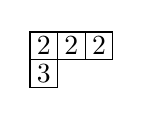
\begin{tikzpicture}[scale=0.35, baseline=-0.5ex]
    \draw (0,0) rectangle (3,1);
    \draw (0,-1) rectangle (1,0);
    \draw (1,-1)--(1,1);
    \draw (2,0)--(2,1);
    \node at (0.5,0.5) {$2$};  \node at (1.5,0.5) {$2$}; \node at (2.5,0.5) {$2$};
    \node at (0.5,-0.5) {$3$};
  \end{tikzpicture}
  }
  +
  \underbrace{x_2^2x_3^2}_{
  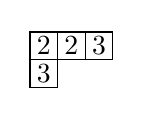
\begin{tikzpicture}[scale=0.35, baseline=-0.5ex]
    \draw (0,0) rectangle (3,1);
    \draw (0,-1) rectangle (1,0);
    \draw (1,-1)--(1,1);
    \draw (2,0)--(2,1);
    \node at (0.5,0.5) {$2$};  \node at (1.5,0.5) {$2$}; \node at (2.5,0.5) {$3$};
    \node at (0.5,-0.5) {$3$};
  \end{tikzpicture}
  }
  +
  \underbrace{x_2x_3^3}_{
  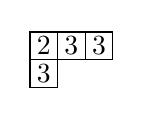
\begin{tikzpicture}[scale=0.35, baseline=-0.5ex]
    \draw (0,0) rectangle (3,1);
    \draw (0,-1) rectangle (1,0);
    \draw (1,-1)--(1,1);
    \draw (2,0)--(2,1);
    \node at (0.5,0.5) {$2$};  \node at (1.5,0.5) {$3$}; \node at (2.5,0.5) {$3$};
    \node at (0.5,-0.5) {$3$};
  \end{tikzpicture}
  }
  \\
  &= x_1^3x_2 + x_1^3x_3 + x_1^2x_2^2 + 2x_1^2x_2x_3 + x_1^2x_2^2 + x_1x_2^3 + 2x_1x_2^2x_3 \\
  &\hspace{1cm}+ 2x_1x_2x_3^2 + x_1x_3^3 + x_2^3x_3 + x_2^2x_3^2 + x_2x_3^3 + x_2x_3^3 \\
  &= m_{(3,1)} + 2m_{(2,1,1)} + m_{(2,2)}
\end{align*}
\end{example}
\end{document}